\documentclass[a4paper]{article}

\usepackage[portuguese]{babel}
\usepackage{comment}
\usepackage[T1]{fontenc}
\usepackage[utf8]{inputenc}
\usepackage{hyperref}
\usepackage{graphicx}
\usepackage{float}
\usepackage{multirow}
\usepackage{indentfirst}
\usepackage[hypcap]{caption} % makes \ref point to top of figures and tables
\usepackage{lscape}
\newcommand{\tab}[1]{\hspace{.2\textwidth}\rlap{#1}}

\graphicspath{ {images/} }

\begin{document}

\begin{titlepage}

	\begin{center}

		
\includegraphics[width=6cm]{./title}\\[3cm]

		\textsc{\LARGE Sistemas de Informação e Bases de Dados}\\[1.5cm]

		\textsc{\Large 1ª Parte do Projeto}\\[1.5cm]


		


		\noindent
		\begin{minipage}{0.4\textwidth}
			\begin{flushleft} \large
				Diogo Proença, 75313
			\end{flushleft}
		\end{minipage}
		\begin{minipage}{0.4\textwidth}
			\begin{flushright} \large
				Diogo Martins, 75462
			\end{flushright}
		\end{minipage}
		
		\begin{minipage}{0.4\textwidth}
			\begin{flushright} \large
				Bernardo Gomes, 75573	
			\end{flushright}
		\end{minipage}

		\vfill

		{\large \today}


	\end{center}

\end{titlepage}
\hypersetup{%
    pdfborder = {0 0 0}
}

\tableofcontents
\pagenumbering{gobble}
\pagebreak
\pagenumbering{arabic}
\section{Modelo E-R}
%explicações do modelo
De acordo com o enunciado, a construção do modelo e-r foi construído de acordo com os seguintes critérios:
\begin{itemize}

	\item as entidades \textit{Medical\_device, Input\_sensor, Actuator, 
	PAN, Pacient e Municipality}, foram retiradas diretamente do enunciado, tal como os respectivos atributos
	
	\item como um \textit{Medical\_device} pode ser tanto um \textit{Input\_sensor} 
	como um Actuator tendo de ser obrigatoriamente pelo menos um deles.
	Desta forma, colocou-se uma especialização total ISA, como se pode verificar no diagrama (duplo traço)

	\item as \textit{weak entities} Readings e Settings foram consideradas como tal, uma vez que tanto uma como a outra não têm o
	conjunto de atributos necessário para servir como \textit{primary key} para a entidades. Assim, assume-se como discriminador 
	o atributo \textit{Physical\_measures} de forma a poder distinguir qual a grandeza medida/lida. Estas entidades são são totalmente
	descritas quando lhe são associadas o \textit{Serial\_number} do \textit{Medical\_device} associado. O atributo \textit{value} é
	\textit{multi-value} pois consoante o dispositivo, o número de parâmetros retirados/lidos é variável. Cada instante de 
	leitura/escrita é 
	armazenado no atributo \textit{time\_instant}
	
	\item a relação \textit{Connects} evidencia a ligação ternária entre as entidades \textit{Medical\_device, PAN} e 
	\textit{Time\_period}. Esta deve-se ao facto de vários \textit{Medical\_devices} se conectarem a um \textit{PAN} (e apenas um),
	 durante um determinado período de tempo. A necessidade de participação da entidade período de tempo, deve-se a possíveis
	 necessidades de remoção de um aparelho (temporaria ou permanentemente)
	 
	\item a relação \textit{Have} representa a ligação ternária entre as entidades \textit{Patient, PAN} e 
	\textit{Time\_period}. Esta deve-se ao facto de um \textit{Patient} se conectar aos seus \textit{Medical\_devices}
	através de um \textit{PAN} (e apenas um \textit{PAN} por \textit{Patient}),
	 durante um determinado período de tempo. A necessidade de participação da entidade período de tempo, deve-se à recuperação de
	 um paciente. Quando este facto ocorre o \textit{PAN} pode também ser atribuído a outro paciente
	 
	 \item as relações ternárias \textit{Lives\_with} e \textit{Lives\_in} mostram a possibilidade de dois pacientes morarem juntos
	 durante certos períodos de tempo e a de um paciente morar num determinado município também durante certo período de tempo
\end{itemize}
\pagebreak
%figura do e-r
\begin{landscape}
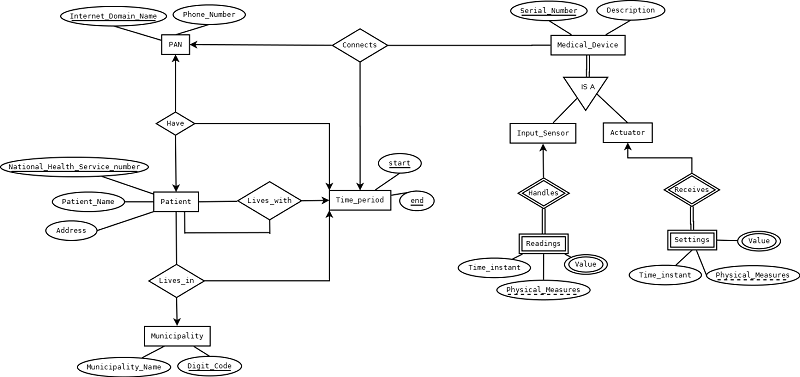
\includegraphics[keepaspectratio]{Diagrama1.png}
\end{landscape}
\pagebreak

\section{Tabelas}
De acordo com o modelo E-R especificado anteriormente, a conversão em tabelas é feita da seguinte forma:

\begin{enumerate}
  \item Conversão de entidades fortes e suas especializações (quando aplicável):
  		\textit{Medical\_device(\underline{Serial}, Description, Internet\_domain\_name)}
  		
  		\textit{Input\_sensor(\underline{Serial})}
  		
  			\tab{Serial:FK(Medical\_device)}
  			
  		\textit{Actuator(\underline{Serial})}
  		
  			\tab{Serial:FK(Medical\_device)}
  		
  		\textit{PAN (\underline{Internet\_domain\_name}, Phone\_number)}
  		
  		\textit{Patient (\underline{National\_health\_service\_number}, Patient\_name, Address, Internet\_domain\_name, Digit\_code, Start, End)}
  		
  				\tab{Internet\_domain\_name:FK(PAN)}
  				
  				\tab{Digit\_code:FK(Municipality)}
  				
  				\tab{Start:FK(Time\_period)}
  				
  				\tab{End:FK(Time\_period)}
  				
  		\textit{Municipality (\underline{Digit\_code}, Municipality\_name)}
  		
  		\textit{Time\_period (\underline{Start}, \underline{End}, Internet\_domain\_name, Digit\_code, Serial\_number)}
  		
  		\tab{Internet\_domain\_name:FK(PAN)}
  				
  		\tab{Digit\_code:FK(Municipality)}
  		
  		\tab{Serial\_number:FK(Medical\_device)}
  		
  		\item Conversão de \textit{weak-entities}:
  		
  		\textit{Readings (\underline{Serial}, \underline{Physical\_measures}, Value, Time\_instant)}
  			
  			\tab{Serial: FK(Input\_sensor)}
  			
  		\textit{Settings (\underline{Serial}, \underline{Physical\_measures}, Value, Time\_instant)}
  			
  			\tab{Serial: FK(Actuator)}
\end{enumerate}

De acordo com a metodologia, seguir-se-ia a conversão de relações e agregações. Porém, sendo as relações presentes no modelo E-R do tipo \textit{one-to-one} ou \textit{many-to-one}, não é necessário a atribuição de uma tabela para a conversão. Esta estará assim presente nas tabelas das suas entidades envolvidas.

De igual forma, por não atribuirmos nenhuma agregação não se construiu qualquer tabela para este conceito.
\end{document}